%=========================================================================
% (c) 2014, 2015 Josef Lusticky

\section{Hardware and networking}\label{sec:setup-hardware}
Figure~\ref{fig:setup-supermicro-board} shows the block diagram of the Supermicro motherboard.
The Intel Xeon E5-2630 v2 processor was plugged into the front CPU socket 00.
To plug the Mellanox ConnectX-3 EN adpater into the PCIE 3.0 x16 slot,
a proprietary Supermicro riser card needed to be used.
The Mellanox ConnectX-3 EN card was then plugged into this riser card.
The front CPU is directly connected to the PCI-Express links, so no QPI links were used in the experiments.
\begin{figure}
	\centering
	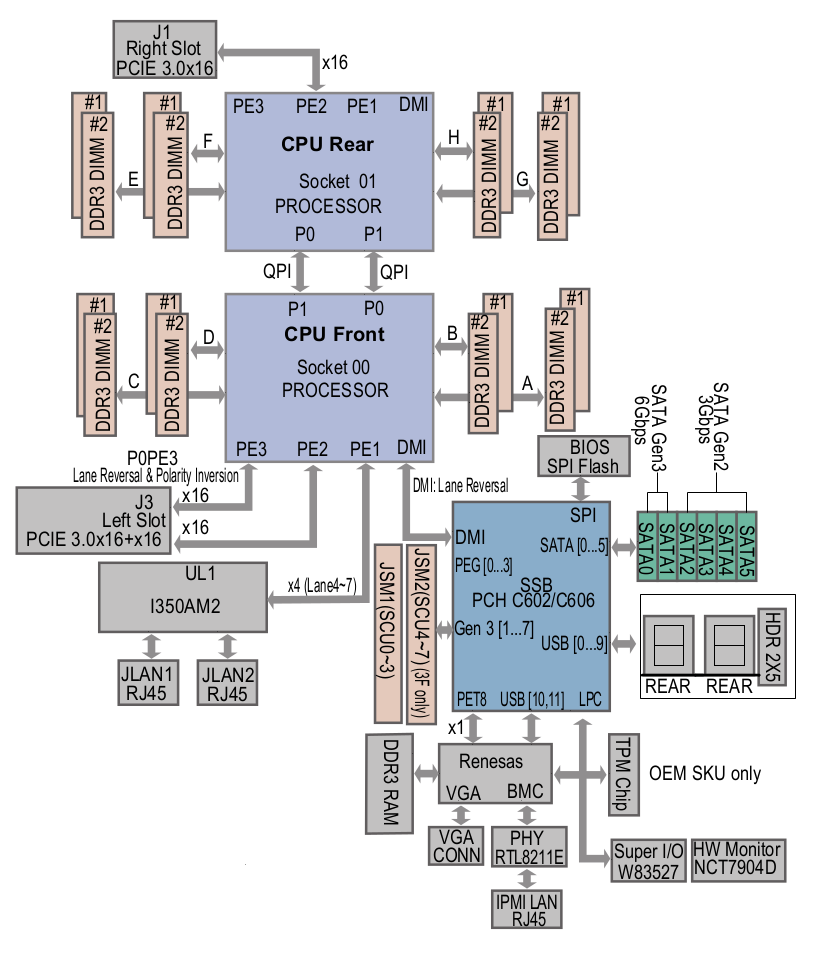
\includegraphics[width=14.5cm,keepaspectratio]{fig/supermicro-board.png}
	\caption{Supermicro motherboard's block diagram}
	\label{fig:setup-supermicro-board}
\end{figure}

The server was put to the same rack as the Spirent hardware generator.
A pair of 40GBASE-SR4 multimode fiber cables with QSPF connectors
was used to connect Spirent with the Mellanox ConnectX-3 EN adapter.

Base CentOS 7 was installed on the server.
The operating system features Linux kernel based on version 3.10 -
the installed version was 3.10.0-123.20.1.el7.x86\_64.
The operating system was updated with all updates avaliable on 7th January 2015.
No external repositories were used. %TODO - check

IPv4 addresses from 192.0.2.0/24 (TEST-NET-1) block were assigned~\cite{rfc5737}.
IPv6 addresses from 2001:db8::/32 range were assigned,
addresses within this block should not appear on the public Internet~\cite{rfc3849}.
Figure~\ref{fig:addressing-scheme} shows the addressing scheme used for the measurements.
\begin{figure}[H]
	\centering
	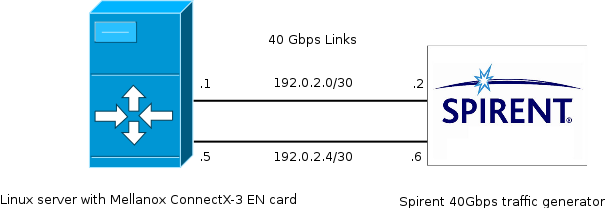
\includegraphics[width=13.5cm,keepaspectratio]{fig/net-setup.png}
	\caption{Addressing scheme}
	\label{fig:addressing-scheme}
\end{figure}



%Enable IPv4 packet forwarding:
%echo 1 > /proc/sys/net/ipv4/ip\_forward


%ip neigh add 1.0.0.2 lladdr f4:52:14:5e:6c:71 dev enp6s0d1
%ip neigh add 2.0.0.2 lladdr f4:52:14:5e:6c:70 dev enp6s0

%ip addr add 1.0.0.1/24 broadcast 1.0.0.255 dev enp6s0d1
%ip addr add 2.0.0.1/24 broadcast 2.0.0.255 dev enp6s0


%Load BGP routes:
%\begin{lstlisting}
%Basic info: size of leaf: 40 bytes, size of tnode: 40 bytes.
%Main:
        %Aver depth:     2.43
        %Max depth:      8
        %Leaves:         503308
        %Prefixes:       538739
        %Internal nodes: 114430
          %1: 58725  2: 26171  3: 14808  4: 7316  5: 4239  6: 2103  7: 1065  8: 2  17: 1
        %Pointers: 995798
%Null ptrs: 378061
%Total size: 61373  kB
%\end{lstlisting}
